% arara: pdflatex
%Began 28 February 2021 --- 
\documentclass[a4paper,x11names,svgnames,10pt]{article}
\usepackage{amsmath}
\usepackage{hyperref}
% the \hypersetup{keyvals} commented out below is stored in an external hyperref.cfg file
% to enable the pagebackref=true option
%\hypersetup{%dvips, % not needed for  pdflatex
%	pagebackref=true,
%	pdfauthor={Iam The Author},
%	hyperfigures,
%	bookmarks=true,
%	bookmarksnumbered=true,
%	bookmarksopen=true,
%	colorlinks=true, %if true, link borders absent
%	pdfborder={1 1 1},
%	citecolor=blue,
%	linkcolor=blue,
%	urlcolor=blue,
%}
\usepackage{url}
\usepackage{svg}
\usepackage{graphicx}
\usepackage{xcolor}
\usepackage{float}
\usepackage{natbib}

\topmargin -0.50in
\oddsidemargin 0.0in
\textwidth 6.27in
\textheight 9.75in

%%%-------------------------------------------
%%% TO BE EDITED FOR EACH NEW VOLUME GENERATED 
%%%-------------------------------------------
	\def\authorName{I Am The Author}
	\def\authorFirstMidNameInit{I.\ T.\ }
	\def\authorLastName{Author}
	\def\dateGenerated{\today}
	\def\volNumber{I}
	\def\mdgBookTitle{Musical Dice Game Waltzes \volNumber}
	\def\mdgBookSubTitle{{\small based on}\\ Der allezeit fertige Polonoisen- und Menuettencomponist (1757) \\ by Johann Philipp Kirnberger}
	\def\theBookSeries{Wonders of the Musical World Series 3}
	\def\theBookPublisher{Libre Edition Press}
	\def\theBookPublisherLogo{../images/1ed.png}
	\def\theBookFrontCover{../images/FrontCover.pdf}
%%%-------------------------------------------
%%%

\def\uline{\underline}
%\definecolor{orange}{rgb}{1,0.5,0} % RGB
%\definecolor{light-gray}{gray}{0.95} % shades
%\definecolor{orange}{cmyk}{0,0.5,1,0} % CMYK

\newcommand{\HRule}{\rule{\linewidth}{0.5mm}}

\setlength{\parindent}{0pt}

\DeclareGraphicsExtensions{.pdf,.png}

\setcitestyle{authoryear,round,comma,aysep={,},yysep={,},notesep={, }}

\title{\textsc{\mdgBookTitle}}
\author{\textsc{\authorFirstMidNameInit \authorLastName}}
\date{\textsc{\dateGenerated}}
% -----

\begin{document}

% Book Cover
% File name: mdgBooSVGV1-title.tex
% Purpose: Book Cover
% Instruction: Should be \input{.} just after \begin{document}
{
\topmargin 0.00in
\oddsidemargin 0.45in
\textwidth 8.27in %letterpaper: 8.50in
\textheight 11.69in %letterpaper: 11.50in
\thispagestyle{empty}

\begin{titlepage}

\begin{picture}(0,0)%
\linethickness{67.00pt}
\color{blue!22!black}
\put(-105,85){\line(1,0){6477}}
\put(-105,-830){\includegraphics[clip=true,trim=0.00in 0.65in 0.25in 0.0in,height=12.50in,width=8.60in,keepaspectratio]%
	{\theBookFrontCover}}
\put(-105,-692){\line(1,0){6477}}
\end{picture}

\vspace{-1.5in}

\begin{center}
	\LARGE\textbf{\color{white} \hspace{-0.5in}\theBookSeries}
\end{center}


\vspace*{3.25\baselineskip}
\begin{center} \Huge\textbf{\color{MediumBlue!1!MidnightBlue}\em \mdgBookTitle}
\end{center}

\vspace{-0.10in}
\begin{center}
	\Large\textbf{\color{MediumBlue!50!MidnightBlue}\em \mdgBookSubTitle}
\end{center}

\begin{center}
	\LARGE\textbf{\color{MediumBlue!25!MidnightBlue}\em compiled by \authorFirstMidNameInit \authorLastName}
\end{center}

\vfill
\begin{center}
	\LARGE\textbf{\hspace{-0.5in}\color{white}\em \theBookPublisher \\ \vspace{-.19in}}
\end{center}
\end{titlepage}
}




\newpage
% Title Page

${}_{}$\\
\vspace{1.00in}	
\thispagestyle{empty}
\begin{center}
	\HRule \\[0.4cm]
	{\huge \bfseries \mdgBookTitle} \\[0.2cm]
	{\large{\em \mdgBookSubTitle} }\\[0.2cm]
	\HRule \\[1.5cm]
	% Author and supervisor
	\begin{minipage}{0.4\textwidth}
		\begin{flushleft} \large
			\emph{Author:}\\
			\authorFirstMidNameInit \textsc{\authorLastName}
		\end{flushleft}
	\end{minipage}
	\begin{minipage}{0.4\textwidth}
		\begin{flushright} \large
			\emph{Supervisor:} \\
			Dr. Communio \textsc{Sanctorum}
		\end{flushright}
	\end{minipage}
	\vfill
	% Bottom of the page
	{\textsc{\Large \theBookSeries}}  \\[0.2cm] 
	\includegraphics*[width=0.15\linewidth]{\theBookPublisherLogo}\\ 
	{\large \theBookPublisher \\
       \dateGenerated }\\
	\vspace{2.50in}
\end{center}
\newpage

%\maketitle		% uncomment if no Front Cover

\tableofcontents\label{tabofcon}

\newpage
%\extrafloats{182}

\section[Introduction]{Introduction\footnote{The information contained in the introduction were culled from the following online resources:
	\citet{wiki_mw2017},\ 
	\url{https://opus-infinity.org/}, and 
	\href{https://www.sciencenews.org/article/mozarts-melody-machine-0}{Mozart's Melody Machine} \citep*{peterson2001}
	}
}
	\begin{center}
	\begin{minipage}{0.4\textwidth}
	\begin{flushleft}
		\begin{center}
			``\em Der \\ allezeit fertige \\ Polonoisen- \\ und \\ Menuetten-componist"\\
		\end{center}
	\end{flushleft}
	\end{minipage}
	\begin{minipage}{0.4\textwidth}
	\begin{flushright}
		\begin{center}
		``\em The \\ Ever-Ready \\ Polonaise \\ and \\ Minuet Composer"
	\end{center}
	\end{flushright}
	\end{minipage}
	\end{center}

Thus is the German title (and its English translation) of the earliest of Musical Dice Games (MDG).  Rightly and interestingly so, as the Instructions provided in the published work allow a non-professional musician to generate (``compose") up to $6^{32} = 7,\!958,\!661,\!109,\!946,\!400,\!884,\!391,\!936$ or nearly eight (8) septillion minuet-trios of which $6^{27} = 1,\!023,\!490,\!369,\!077,\!469,\!249,\!536$ or about one (1) sextillion are unique (see Subsection~\ref{tableFind} for more details).\\  

A {\it Musikalisches W\"{u}rfelspiel} (German for ``musical dice game" or MDG) is a system for randomly ``generating" (e.g., by using a die or two dice) musical compositions from precomposed options and was quite popular throughout Western Europe in the 18th century. Aside from Kirnberger's {\em Der allezeit fertige Polonoisen- und Menuettencomponist} ({\it 1st ed.\ 1757; rev.\ 2nd ed.\ 1783}), other well-known composers that are to known to have composed  (or have been attributed the composition of) a MDG are Wolfgang Amadeus Mozart ({\em Anleitung zum Componieren von Walzern so viele man will vermittelst zweier Würfel, ohne etwas von der Musik oder Composition zu verstehen}---German for ``Instructions for the composition of as many waltzes as one desires with two dice, without understanding anything about music or composition"), C.P.E.\ Bach ({\em Einfall, einen doppelten Contrapunct in der Octave von sechs Tacten zu machen, ohne die Regeln davon zu wissen} ({\it 1758}); translated from German as ``A method for making six bars of double counterpoint at the octave without knowing the rules") and Abb\'{e} Maximillian Stadler ({\em Table pour composer des minuets et des Trios \`{a} la infinie; avec deux dez \`{a} jouer} ({\it 1780}); translated from French as ``A table for composing minuets and trios to infinity, by playing with two dice"). \\

{\it Musikalisches W\"{u}rfelspiel K.\ 516f} ({\it 1787}), another title for the MDG attributed to Mozart and is the most famous of MDGs, was first published by J.J. Hummel in 1793 in Berlin, and was republished in 1796 by Nikolaus Simrock in Bonn (as {\em K.\ 294d} or {\em K.\ Anh.\ C 30.01}).  Simrock attributed this work to Mozart and it may have been based on Mozart's manuscript {\em K.\ 516f}, written in 1787, consisting of numerous two-bar fragments of music, that appear to be some kind of game or system for constructing music out of two-bar fragments, but contains no instructions nor hints as to the use of dice.  An \href{(http://www.asahi-net.or.jp/\~rb5h-ngc/e/k516f.htm}{online article} by Hideo Noguchi offers a possible explanation for this attribution. \\

This book is a collection of 28 MDG minuet-trios generated according to the rules given in {\it Der allezeit fertige} (we will refer to this MDG in this manner from here onward).  The scores of the generated minuet-trios, that were initially written using the \texttt{abc} environment of Chris Walshaw, were converted to Scalar Vector Graphics (SVG) images (with corresponding MIDIs) by using {\tt abcm2ps} and {\tt abcmidi}, and were then pre-processed with Inkscape to be included in \LaTeX\ to produce this book.


\section{\em Der allezeit fertige}

\subsection{Rules}

The Rules provided in {\it Der allezeit fertige} generate MDG minuets-trios consisting of 32 bars (or measures), 16 bars each for the minuet and trio sections.  For each of these two sections, the first eight (8) bars are played then repeated.  The last eight bars are then similarly played. Finally, the 16 bars of the minuet are again played but without repeats for each set of 8 bars. \\

The following Rules are followed for generating each minuet:
\begin{enumerate}
	\item [1.] For each bar from the first to the 16th, a regular six-sided die is tossed and the face that comes up is obtained.  Hence, 16 one-die tosses (with possible outcomes from the set \{1, 2, 3, 4, 5, 6, \}), a toss of a die for each bar, are needed to generate a minuet section.   
	\item [2.] Table~\ref{fig:0tab1}(a) is then used to determine which bar number from the Table of Measures for Minuets (Figures~\ref{fig:meas1} to \ref{fig:meas2}) is to be used for obtaining the notes---based on the outcome of each one-die toss---for the particular bar of the minuet-to-be-generated.  The possible outcomes of a die toss (1 to 6) are given on the left-hand side (stub items) of Table~\ref{fig:0tab1}, while the bar numbers of the minuet-to-be-generated are given on the top of that table (captions or column  headings).
	\item [3.]  For example, suppose for bar 1, the outcome of the two-dice toss is 5.  If we now look for bar number 1 at the top of Table~\ref{fig:0tab1} and for the outcome 5 on the left-hand side of that table, we obtain 43 as the measure number of the Table of Measures for Minuets (see Figure~\ref{fig:meas1}) to be used for obtaining the notes to be played for the first bar of the minuet-to-be-generated.  Similarly, an outcome of 4 for the one-die toss for bar 9 of the minuet-to-be-generated leads us to obtain the notes from bar 95 of the Table of Measures for Minuets (see Figure~\ref{fig:meas2}).
\end{enumerate}   

The following Rules are followed for generating each trio:
\begin{enumerate}
	\item [1.] For each bar of the trio, from the first bar to the 16th, a die is tossed.  Hence, 16 one-die tosses with possible outcomes from the set \{1, 2, 3, 4, 5, 6\}, a toss of a die for each bar, are needed to generate a trio.   
	\item [2.] Table~\ref{fig:0tab1}(b) is then used to determine which bar number from the Table of Measures for Trios (Figures~\ref{fig:meas3} to \ref{fig:meas4}) is to be used for obtaining the notes, based on the outcome of each die toss, for the bar of the trio corresponding to that one-die toss .  The possible outcomes of a toss of a die (1 to 6) are given on the left-hand side  (stub items) of Table~\ref{fig:0tab1}(b), while the measure numbers of the minuet-to-be-generated are given on the top of that table (captions or column  headings).
	\item [3.]  For example, suppose for bar 1, the outcome of the one-die toss is 3.  If we now look for measure number 1 at the top of Table~\ref{fig:0tab1} and for the outcome 3 on the left-hand side of that table, we obtain 8 as the bar number of the Table of Measures for Trios (see Figure~\ref{fig:meas3}) to be used for obtaining the notes to be played for the first measure of the trio-to-be-generated.  Similarly, an outcome of 1 on the one-die toss for bar 9 of the trio-to-be-generated leads us to obtain the notes from bar 94 of the Table of Measures for Trios (see Figure~\ref{fig:meas5}) .
\end{enumerate}   


\subsection{Table for finding Measure Number from Table of Measures}\label{tableFind}
The table given here (Table~\ref{fig:0tab1}) combines the two tables given on pages 9 and 10 of {\it Der fertige allezeit} but the contents are exactly as given there with the roles of the rows and columns switched.  The leftmost column contains the possible one-die outcomes while the topmost row contains the bar number for the MDG minuet/trio to be generated. 

\begin{table}[H]
	\centering
	\begin{tabular}{c}
		\centering
		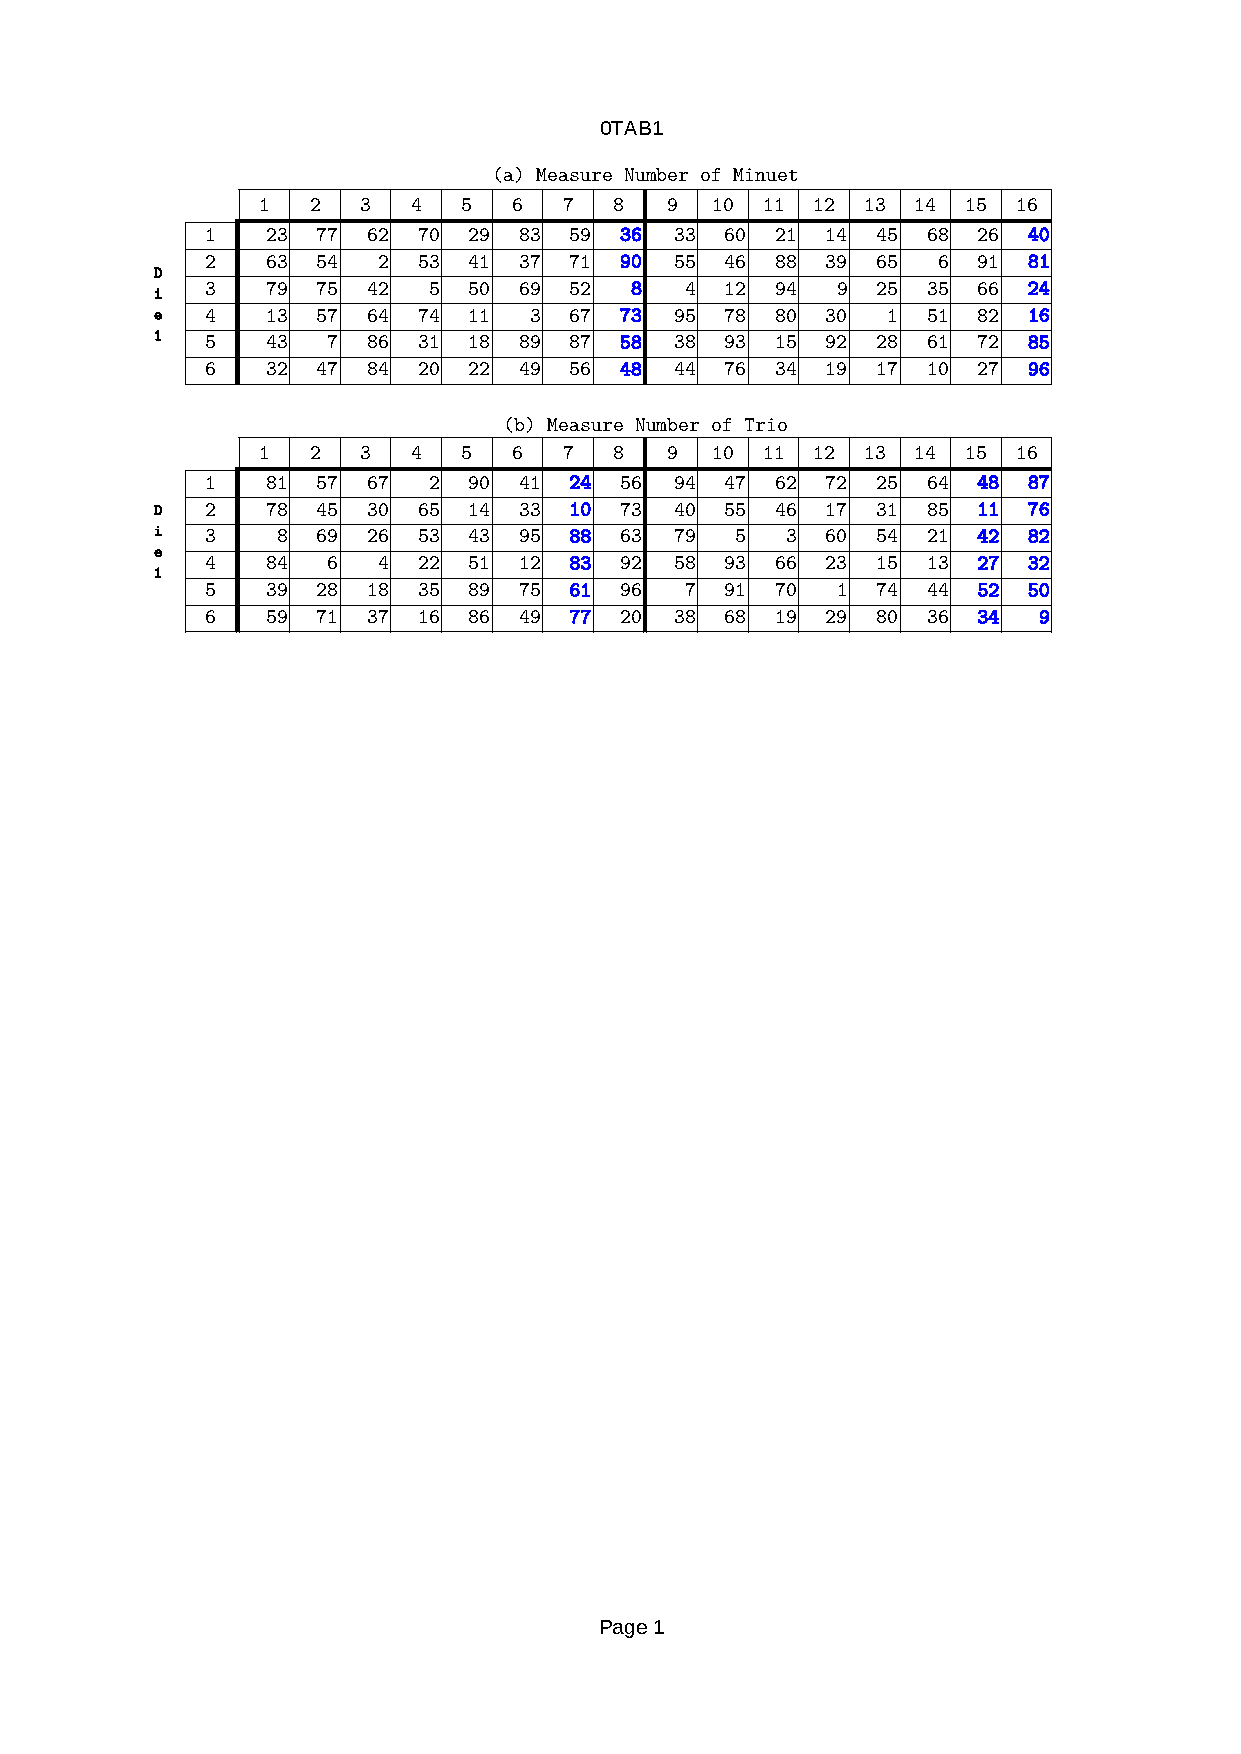
\includegraphics[clip=true,trim=0.90in 7.45in 1.25in 1.00in,scale=0.90]{012TAB}
	\end{tabular}
	\caption{Measure number to be looked-up in the Table of Measures (see Figures~\ref{fig:meas1}, \ref{fig:meas2}, \ref{fig:meas3}, \ref{fig:meas4}, and \ref{fig:meas5} in Section~\ref{tableMeas}) corresponding to each one-die outcome per bar for the minuet and trio. Measure number in {\bf\color{blue}bold blue font} indicates identical measures under that column (see  \href{https://opus-infinity.org/dice_games/kirnberger_menuet_trio/tables/}{https://opus-infinity.org} for more info).}
	\label{fig:0tab1}
\end{table}

Although the body of Table~\ref{fig:0tab1} includes $6\times 16 + 6\times 16 = 192$ bar numbers, the Tables of Measures for Minuets and Trios (Figures~\ref{fig:meas1} to \ref{fig:meas4}) contain only $6\times 14 + 6\times 13 + 5 = 167$ different measures.  This is so since in Table~\ref{fig:0tab1}: a) for the minuet bars, all the measures under bar 8 and all the measures under bar 16 are identical giving only two (2) unique measures; b) for the trio bars, all the measures under bar 7 and all the measures under bars 15 and 16 are identical, giving three (3) unique measures; c) there are six (6) different measures for each of the remaining 14 bars of the minuet and six (6) diffrent measures for each of the remaining 13 bars of the trio: $6\times 14 + 6\times 13 = 162$ additional bars.  These also explain why the total number of unique minuet-trios that can be generated is $(6^{14}\times 6^{13}\times 1\times 1\times 1\times 1\times 1) = 6^{27}.$

\nopagebreak[4]
\subsection{Table of Measures}\label{tableMeas}

\addcontentsline{toc}{subsection}{\hspace*{0.25in}{\em Der allezeit fertige} page 1 of measures}
\begin{figure}[H]
	\centering
	\def\svgwidth{0.975\columnwidth}
	\input{knbgr-easy-minuet001.pdf_tex}
	\caption{Table of Measures for Minuets (Part I)}
	\label{fig:meas1}
\end{figure}

\newpage
${}_{}$\\
\vspace{0.10in}
\addcontentsline{toc}{subsection}{\hspace*{0.25in}{\em Der allezeit fertige} page 2 of measures}
\begin{figure}[H]
	\centering
	\def\svgwidth{0.975\columnwidth}
	\input{knbgr-easy-minuet002.pdf_tex}
	\caption{Table of Measures for Minuets (Part II)}
	\label{fig:meas2}
\end{figure}

\newpage
${}_{}$\\
\vspace{0.10in}
\addcontentsline{toc}{subsection}{\hspace*{0.25in}{\em Der allezeit fertige} page 3 of measures}
\begin{figure}[H]
	\centering
	\def\svgwidth{0.975\columnwidth}
	\input{knbgr-easy-trio001.pdf_tex}
	\caption{Table of Measures for Trios (Part III)}
	\label{fig:meas3}
\end{figure}

\newpage
${}_{}$\\
\vspace{0.10in}
\addcontentsline{toc}{subsection}{\hspace*{0.25in}{\em Der allezeit fertige} page 4 of measures}
\begin{figure}[H]
	\centering
	\def\svgwidth{0.975\columnwidth}
	\input{knbgr-easy-trio002.pdf_tex}
	\caption{Table of Measures for Trios (Part IV)}
	\label{fig:meas4}
\end{figure}

\newpage
${}_{}$\\
\vspace{0.10in}
\addcontentsline{toc}{subsection}{\hspace*{0.25in}{\em Der allezeit fertige} page 5 of measures}
\begin{figure}[H]
	\centering
	\def\svgwidth{0.975\columnwidth}
	\input{knbgr-easy-trio003.pdf_tex}
	\caption{Table of Measures for Trios (Part V)}
	\label{fig:meas5}
\end{figure}


\newpage
\section{Related Links}
The following are very interesting sites in that they allow the online rendering of MDGs:
\begin{itemize}
	\item  \href{https://marian-aldenhoevel.de/mozart/}{Mozart} - A site maintained by Marian Aldenh\"{o}vel allows the visitor to generate a MDG (user-specified or randomly-generated) and the corresponding audio ({\tt midi, wav}) and image files ({\tt PDF, PNG}) based on {\em Musikalisches W\"{u}rferspiel, K.\ 516f}.
	
	\item \href{https://opus-infinity.org}{Opus Infinity} - Collaborative work of Robbert Harms, Hein Moors, and Suus van Petegem whose goal is to unravel the mystery behind the tables used for generating MDGs.  Site visitors can generate MDGs based on works of Kirnberger, Mozart, Stadler/Haydn, and Bach.  Corresponding audio files ({\tt mid, ogg,} and/or {\tt mp3}) and image files ({\tt PDF} or {\tt PNG}) are also made available for listening, viewing, or downloading.
	
	\item  \href{http://sunsite.univie.ac.at/Mozart/dice/}{Mozart} - A site maintained by John Chuang that allows the site visitor to generate MDGs based on the work of Stadler/Haydn.
 	
 	\item \href{https://www.amaranthpublishing.com/mozart.zip}{\tt mozart.zip} -  This is a Windows software (\textcopyright 1995 VisionSoft) by John Chuang and Stephen Goodwin that generates MDG based on input from user and is available for {\it free} from  \href{http://www.amaranthpublishing.com/MozartDiceGame.htm}{Amaranth Publishing}.  
 	
 	\item \href{http://www.asahi-net.or.jp/\~rb5h-ngc/e/k516f.htm}{``Mozart - Musical Game in C K. 516f,"}	Mozart Studies Online - The site of Hideo Noguchi that offers an explanation linking {\em Musikalisches W\"{u}rferspiel, K.\ 516f}, and  {\em K.\ 294d (K.\ Anh.\ C 30.01)}. 
\end{itemize}

\section{Acknowledgments}
My sincerest gratitude to Chris Walshaw et al. for the \href{http://www.abcnotation.com/}{ABC music notation}; Jean-Francois Moine for \href{http://moinejf.free.fr/}{\tt abcm2ps} and the accompanying examples, templates, and pointers for the appropriate use of these resources; Guido Gonzato for the \href{http://abcplus.sourceforge.net/}{ABC Plus Project} and the \href{http://abcplus.sourceforge.net/#abcMIDI}{{\tt abcmidi} resources} available there, more especially for the ABC resource book {\em Making Music with ABC 2}; James R. Allwright and Seymour Shlien for \href{http://abc.sourceforge.net/abcMIDI}{\tt abcmidi} source and binaries; \href{https://artifex.com/}{Artifex, Inc.} for Ghostscript v.10.00.0 (includes the {\tt ps2pdf} converter); \href{https://www.inkscape.org/}{Inkscape v.1.2.2} for the tool for converting SVGs to PDFs for inclusion into \LaTeX\ documents; William Schelter for \href{https://maxima.sourceforge.io}{Maxima v.5.47.0}---used for computing the permutation number; Colomban Wendling et.\ al for \href{https://www.geany.org}{Geany 2.0 IDE}; and \href{https://tex.stackexchange.com/users/632/martin-h}{\tt User:Martin H} for his \href{https://tex.stackexchange.com/questions/2099/how-to-include-svg-diagrams-in-latex}{reply} to a \TeX\ / \LaTeX\ Stack Exchange question on including SVGs into \LaTeX\ documents. Special thanks also to the \href{http://imslp.org/}{International Music Score Library Project (IMSLP)} for making available the score for {\it Der allezeit fertige Polonoisen- und Menuettencomponist} ({\it 1757}) and \href{http://www.amaranthpublishing.com/MozartDiceGame.htm}{Amaranth Publishing} for a copy of {\tt mozart.zip}. Ditto to Machtelt Garrels for the book \href{http://tldp.org/LDP/Bash-Beginners-Guide/html/Bash-Beginners-Guide.html}{Bash Guide for Beginners}, Vivek Gite for the book \href{http://www.freeos.com/guides/lsst/}{Linux Script Shell Tutorial}, and Steve Parker for the \href{http://steve-parker.org/sh/cheatsheet.pdf}{Unix/Linux Shell Cheatsheet}. John Fogarty's GitHub Site: \href{https://github.com/jfogarty/latex-createspace-bookcover}{Latex CreateSpace BookCover} and Peter Wilson's reply in \TeX\ / \LaTeX\ Stack Exchange on \href{https://tex.stackexchange.com/questions/17579/how-can-i-design-a-book-cover}{designing a book cover}, were sources of ideas, information, and materials for creating the book cover and title page, thanks to both of them; \href{http://www.libreoffice.org/}{LibreOffice Calc} for its use in the image creation of the book cover.  Many thanks, too, to the \href{https://www.debian.org}{Debian Project} for the Debian 12 (Bookworm) GNU/Linux OS,\href{http://www.tug.org/texlive/}{TeXLive 2024} for providing the \TeX\ distribution,  and \href{https://github.com}{GitHub} for its generosity in providing space for \href{https://github.com/justineuro/mdgBookSVG3Kit}{the project}.

\newpage
\section{Selected Waltzes}
%\vspace{0.80in}
\vspace{-.10in}
{
\small
\topmargin -1.00in
\textheight 10.25in
	\input{svgList}
}	

\newpage
\section{License}
This work by I Am The Author, based on work of J.L.A. Uro at  \url{https://github.com/justineuro/mdgBookSVG3Kit}, is licensed under a Creative Commons Public Domain International License.

\bibliographystyle{plainnat}
\bibliography{mdg4}

 

\end{document}
